% ============================================================================
\section{Results}
\label{sec:results}
% ============================================================================
\subsection{Recalculation Under Retroactive Rules}
\label{sec:res-retro}
The payroll as known before the upload stayed unchanged in all 15 late-upload scenarios (Table~\ref{tab:late}), as the append-only records of the knowledge base guarantee. The employer can therefore still reproduce what was withheld at the time. The reference updates changed the paid withholding of 3,276 employee-months summed over the scenarios. The affected test cases ranged from one under the tourism extension of E10 to about 250 under the rounding rule of E13. Cases in the table are test employee-years whose paid withholding or annual values change under the reference update, and paid months are the changed months already paid. The report covered more months the longer the upload was delayed. No code was changed in any scenario.

\begin{table}[!t]
\caption{Late upload of the five retroactive rules.}
\label{tab:late}
\centering\footnotesize
\setlength{\tabcolsep}{3pt}
\begin{tabularx}{\columnwidth}{@{}lLrrc@{}}
\toprule
Event & Retroactive rule & Cases & Paid months, lag 1/2/3 & Report \\
\midrule
E06 & DTP for labor-intensive industry, 2025 & 24 & 20/21/35 & $\times\,\times\,\times$ \\
E07 & 50\% relief of the work-accident premium & 43 & 33/66/99 & \checkmark\,\checkmark\,\checkmark \\
E09 & extension of the premium relief & 34 & 68/102/136 & \checkmark\,\checkmark\,\checkmark \\
E10 & DTP extended to tourism & 1 & 1/2/3 & \checkmark\,\checkmark\,$\times$ \\
E13 & rounding to the nearest rupiah & 249--250 & 751/898/1,041 & \checkmark\,\checkmark\,\checkmark \\
\midrule
Sum & 15 scenarios (earlier payroll reproducible in all) & & 3,276 & 11 of 15 \\
\bottomrule
\end{tabularx}
\end{table}

The system's own recalculation report equaled the reference report in 11 of the 15 scenarios (report column of Table~\ref{tab:late}). All nine scenarios of the three events whose drafted update was correct (E07, E09, E13) matched exactly, among them the three scenarios of the rounding rule with up to 1,041 paid employee-months. The four differences came from the two updates that were already wrong in the isolated mode. The E06 update differed at every lag. The one wrong value of the E10 update fell in a month already paid only at the longest lag. The bitemporal representation thus turned a correct update into a correct retroactive correction at each of the three upload lags.

\subsection{Single Updates}
\label{sec:res-single}
In the isolated mode (Fig.~\ref{fig:outcomes}) the system made 41 correct updates and 15 silent errors (SER 0.19, one-sided upper bound 0.27) on the 80 prospective units and abstained on 24. Of the 39 updates proposed for regulation units, 35 were correct and 4 were silent errors. Parameter changes (T1) and changes of calculation method (T7) were correct in all 13 units of these types. Company-policy units were harder, with 6 of 30 correct, 13 abstentions, and 11 silent errors. Five of these 11 silent errors only named the amended policy differently from the reference. When the policy identifiers of memo updates were mapped to the policy in force, the prospective outcomes became 46 correct updates, 24 abstentions, and 10 silent errors.

The system drafted 9 of the 13 real regulations correctly and abstained on 2 of them and on all six labor agreements. A second run gave the same outcome for 12 of the 13 regulations. None of the 20 distractors changed a payslip: the system judged 13 of them not relevant, abstained on 5, and drafted updates without any effect for the other 2. Fig.~\ref{fig:outcomes} counts these 13 and 2 distractors as correct.

\begin{figure}[!t]
\centering
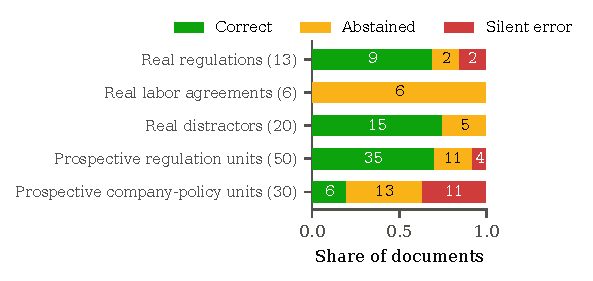
\includegraphics[width=\columnwidth]{figs/fig_outcomes.pdf}
\caption{Outcome of single updates in the isolated mode.}
\label{fig:outcomes}
\end{figure}

Among the baselines built from the same drafts (Table~\ref{tab:single}), the behavioral majority of all drafts without gates (B4) applied the selection rule of the closest work and made 24 silent errors on the prospective set and 2 on the real labor agreements. Every selection that used the gates made 13 to 15. The schema and quote checks alone (B3) already account for this reduction. The consensus did not add to it: the first draft that passes all gates (B2) was as accurate as the upper bound and made 43 correct updates against 41 for the system. The difference in correct updates between the system and B3 was $+0.025$ (95\% interval $-0.023$ to $0.072$). Each cell of Table~\ref{tab:single} gives correct updates, abstentions, and silent errors in this order.

\begin{table}[!t]
\caption{Single updates of the system and the baselines built from the same drafts.}
\label{tab:single}
\centering\footnotesize
\setlength{\tabcolsep}{3pt}
\begin{tabular}{@{}lccc@{}}
\toprule
Selection & Prospective & Regulations & Agreements \\
 & (80) & (13) & (6) \\
\midrule
System & 41 / 24 / 15 & 9 / 2 / 2 & 0 / 6 / 0 \\
B2, first passing draft & 43 / 23 / 14 & 10 / 2 / 1 & 0 / 6 / 0 \\
B3, first draft passing G1--G2 & 39 / 28 / 13 & 8 / 3 / 2 & 0 / 6 / 0 \\
B4, majority without gates & 41 / 15 / 24 & 10 / 2 / 1 & 0 / 4 / 2 \\
Upper bound & 43 / 23 / 14 & 10 / 2 / 1 & 0 / 6 / 0 \\
\bottomrule
\end{tabular}
\end{table}

Claude Sonnet 5.5 as drafting model gave 26 correct updates, 6 abstentions, and 7 silent errors on the 39 real documents, against 24, 13, and 2 for \texttt{gpt-6.1-sol}. The two models agreed on 29 of the 39 documents ($\kappa = 0.52$) and on 12 of 20 prospective units ($\kappa = 0.40$). Sonnet abstained less often and accepted two distractors as changes.

\subsection{Payslip Accuracy of Companies Over Time}
\label{sec:res-chain}
In the reviewer condition, payslip accuracy on the payroll date (Fig.~\ref{fig:payslip} and Table~\ref{tab:chain}) was 0.978 at Company A, 0.961 at Company B, 0.945 at Company C, and 1.000 at Company E. In each of these four companies the share of correct payslips exceeded that of the code-based update by about two to three percentage points. This margin arose because the system brought each correct regulation into the payroll on its issue date instead of 26 days later. This advantage is confined to the payslips whose payroll date falls within 26 days after an issue. Accuracy at Company D was 0.239, which Section~\ref{sec:res-gate} traces to a single proposal. Accuracy pooled over the five companies was 0.842 against 0.951 for the code-based update. The series with the completeness gate in Figs.~\ref{fig:payslip} and~\ref{fig:monthly} belong to the design iteration of Section~\ref{sec:res-gate}.

The code-based update and the reviewer condition lose payslips in different months (Fig.~\ref{fig:monthly}). At Companies A, B, and C the code-based update loses all or nearly all payslips of February and September 2025 and part of those of May 2025 and January 2026, the months whose payroll date falls within the 26 days after a change. The reviewer condition loses payslips mostly in December, when the year is recomputed. Company B also loses February 2025 in this condition because the engineer's update for E06 arrived after the payroll date. At Company D the reviewer condition loses every payslip from April 2024 to March 2026, whereas the completeness gate keeps Company D correct in every month.

\begin{figure*}[!t]
\centering
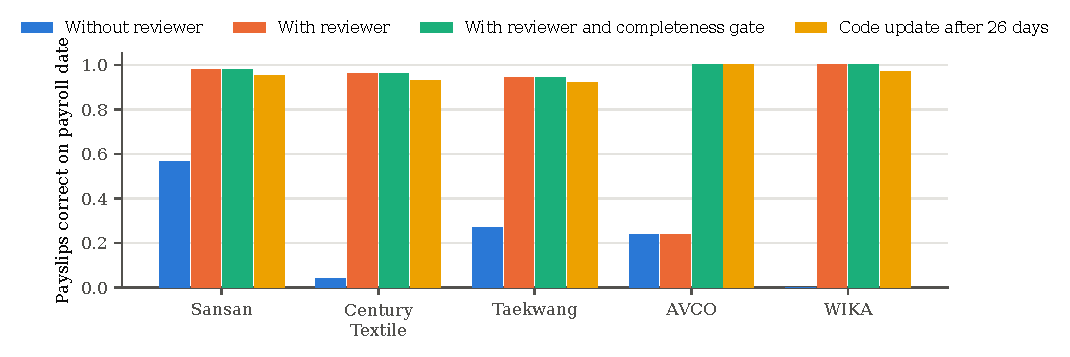
\includegraphics[width=0.92\textwidth]{figs/fig_payslip.pdf}
\caption{Payslip accuracy on the payroll date in the five real companies under each condition.}
\label{fig:payslip}
\end{figure*}

\begin{figure*}[!t]
\centering
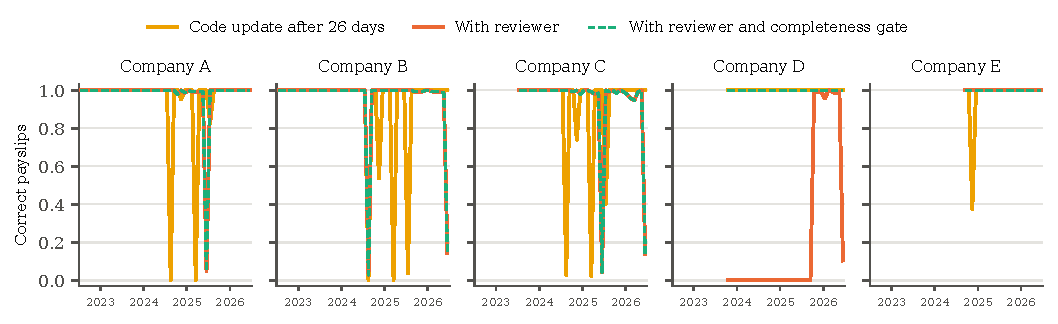
\includegraphics[width=0.95\textwidth]{figs/fig_monthly.pdf}
\caption{Monthly payslip accuracy on the payroll date in the five real companies.}
\label{fig:monthly}
\end{figure*}

\begin{table*}[!t]
\caption{Payslips, documents, engineer-written updates, accuracy, and cost of the chained mode.}
\label{tab:chain}
\centering\footnotesize
\setlength{\tabcolsep}{3pt}
\resizebox{\textwidth}{!}{%
\begin{tabular}{@{}lrrrrrrrrrrr@{}}
\toprule
 & & & Written by & \multicolumn{4}{c}{Accuracy on the payroll date} & \multicolumn{3}{c}{Accuracy at the end of the window} & \\
\cmidrule(lr){5-8}\cmidrule(lr){9-11}
Company & Payslips & Documents & engineer & Without reviewer & Reviewer & Careful reviewer & Code-based & Reviewer & Careful reviewer & Code-based & Cost (USD) \\
\midrule
Company A & 7,026 & 34 & 3 & 0.566 & 0.978 & 0.994 & 0.953 & 0.978 & 1.000 & 1.000 & 8.57 \\
Company B & 6,747 & 35 & 5 & 0.041 & 0.961 & 0.954 & 0.930 & 0.981 & 0.986 & 1.000 & 9.64 \\
Company C & 5,039 & 27 & 1 & 0.268 & 0.945 & 0.967 & 0.922 & 0.945 & 1.000 & 1.000 & 4.68 \\
Company D & 4,558 & 25 & 0 & 0.239 & 0.239 & 0.239 & 1.000 & 0.239 & 0.239 & 1.000 & 4.39 \\
Company E & 2,958 & 17 & 2 & 0.000 & 1.000 & 1.000 & 0.969 & 1.000 & 1.000 & 1.000 & 3.83 \\
\midrule
Real companies, pooled & 26,328 & 138 & 11 & 0.254 & 0.842 & 0.849 & 0.951 & 0.847 & 0.865 & 1.000 & 31.11 \\
\midrule
Simulation A (5 companies) & 33,175 & 43 & 6 & 0.651 & 0.911 & 0.942 & 0.986 & 0.911 & 0.939 & 1.000 & 9.87 \\
Simulation B (5 companies) & 33,199 & 43 & 4 & 0.844 & 0.824 & 0.958 & 0.993 & 0.824 & 0.958 & 1.000 & 8.46 \\
\bottomrule
\end{tabular}}
\end{table*}

The end of the window shows the cost of the silent errors. The code-based update is correct by construction once it arrives and reached 1.000 everywhere, whereas the system kept the effect of its silent errors and ended at 0.945 to 1.000 in the four companies. The careful-reviewer condition raised the end-of-window accuracy to 1.000 at Companies A and C by rejecting each proposal whose review payslips differ from those of the reference update. At Company B it scored lower on the payroll date than the reviewer condition (0.954 against 0.961) because each rejected proposal is replaced by an update written 26 days after issue.

The engineer wrote the update by hand for 11 of the 138 documents that the five companies received (Fig.~\ref{fig:workload}), each time after an abstention. The other 14 abstentions concerned documents without effect on the payroll. The figure also counts the 59 documents judged not relevant and the 11 proposals without effect on any payslip. The system decided the remaining 113 documents at a model cost of about USD 0.23 per document. The 54 steps that carried a real change comprised 33 correct proposals, 11 updates written by the engineer, and 10 silently wrong proposals that the reviewer condition approved. The labor agreements that install the company layer were the weak point: the engineer wrote five of the six, and the sixth was the incomplete proposal for Company D. These abstained installations also explain the low accuracy without a reviewer (0.000 at Company E and 0.041 at Company B) because the company layer then stays empty.

\begin{figure*}[!t]
\centering
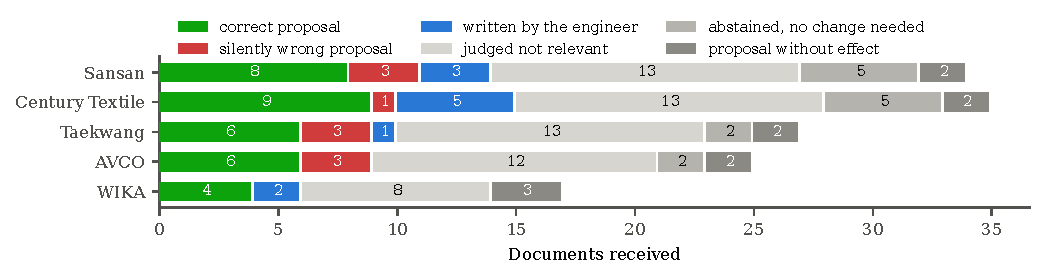
\includegraphics[width=0.92\textwidth]{figs/fig_workload.pdf}
\caption{Decision on each document received by the five real companies.}
\label{fig:workload}
\end{figure*}

The simulation chains confirm that unchecked company-policy proposals carry the most risk. Their fictional companies received synthetic policy memos, the type of document that was hardest in the isolated mode. Both chains stayed below the code-based update in the reviewer condition. In Simulation B approving every proposal (0.824) was worse than leaving every abstention unhandled (0.844). The careful-reviewer condition recovered most of the gap in Simulation B and about two fifths of it in Simulation A.

\subsection{Error Propagation and Pre-Specified Hypotheses}
\label{sec:res-hyp}
In 40 of the 48 pairs of a regulation and a real company, the update in the chain had the same outcome as the first isolated run of the same regulation. Four pairs improved in the chain, where a silent error of the isolated run became a correct update or an abstention. The 2026 DTP regulation (E11) went the other way: it was correct in both isolated runs but wrong in four of the five chains. E11 extends the facility rules of E06 and E10. In the chains it was drafted against the system's own knowledge base, whose earlier updates differed from the reference. Which difference triggered the error was not isolated. The labor agreement of Company D adds a ninth discrepancy because the system abstained on it in isolation but proposed an update in its chain.

H1 is not supported (Table~\ref{tab:hyp}). The reviewer condition differed from the code-based update by $-0.109$ pooled over the five real companies (95\% interval $-0.345$ to $0.030$ over 54 event--chain clusters). This result was driven by Company D, without which the difference was $+0.027$. E11 also meets the pre-specified definition of systematic propagation.

On the prospective set the SER of 0.19 exceeded its threshold of 0.15, and the system made 15 silent errors against 13 for B3. H2 is therefore not supported either, although the abstention rate of 0.30 met its threshold.

\begin{table}[!t]
\caption{Pre-specified hypotheses and their outcomes.}
\label{tab:hyp}
\centering\footnotesize
\setlength{\tabcolsep}{3pt}
\begin{tabularx}{\columnwidth}{@{}Lll@{}}
\toprule
Criterion & Threshold & Result \\
\midrule
H1(a) accuracy vs code-based update & bound $> -0.01$ & $-0.109$ [$-0.345$, $0.030$] \\
H1(b) systematic propagation & none & E11 \\
H2(a) SER, prospective set & bound $\leq 0.15$ & 0.19 (bound 0.27) \\
H2(b) SER lower than B3 & McNemar $p < 0.05$ & 15 vs 13, $p = 0.89$ \\
H2(c) abstention rate & $\leq 0.50$ & 0.30 \\
\bottomrule
\end{tabularx}
\end{table}

\subsection{Design Iteration: A Completeness Gate}
\label{sec:res-gate}
The chain of Company D starts with the installation of its labor agreement. The proposal for this document declared two facts (a base salary and a radiation allowance) and added no rule that used them. The draft's own note stated that the update was not computationally complete. Such a proposal passes every gate because G5 checks the effect of rules and skips facts. Without any effect, the proposal also shows no difference on the review page. Payslip accuracy at Company D stayed at 0.239 until the end of the window because the approved proposal left the pay clauses of the agreement out of the payroll.

This failure led to a completeness gate G7 that was defined after the measured runs. G7 requires a draft for a document judged relevant to change at least one observed value, conflict, or engine error on its own review cases. The rule was written down before it was applied to any test data and was checked first on the 100 passing drafts of the development runs, where it changed no outcome. It was then replayed on the recorded drafts of the measured runs with the same random order, without a repair round, and without new model calls. Accuracy at Company D rose from 0.239 to 1.000 while the other companies were unchanged (Table~\ref{tab:gate}). The system with the completeness gate matched or exceeded the code-based update in all five companies. The pooled difference became $+0.022$ (95\% interval $-0.006$ to $0.052$), but H1 remains unsupported because E11 still propagates.

The gate also turned 10 updates that were scored correct into abstentions. Two of them were the distractor updates without effect, which the gate is meant to stop. The other eight were correct regulation updates whose effect the review cases did not reach, such as an effect that starts in a month after the issue. On the prospective set the share of correct updates fell from 0.51 to 0.41 and the abstention rate rose from 0.30 to 0.40 without any change in silent errors. In the chains the system decided 73\% of the documents instead of 82\%, and the engineer wrote 12 updates instead of 11.

\begin{table}[!t]
\caption{Effect of the completeness gate G7 on the recorded drafts.}
\label{tab:gate}
\centering\footnotesize
\setlength{\tabcolsep}{3pt}
\begin{tabularx}{\columnwidth}{@{}Lrr@{}}
\toprule
Measure & Without G7 & With G7 \\
\midrule
Company D payslip accuracy, payroll date & 0.239 & 1.000 \\
Companies at or above the code-based update & 4 of 5 & 5 of 5 \\
Pooled difference to the code-based update & $-0.109$ & $+0.022$ \\
95\% interval of the difference & [$-0.345$, $0.030$] & [$-0.006$, $0.052$] \\
Systematic propagation (H1(b)) & E11 & E11 \\
Pooled accuracy at the end of the window & 0.847 & 0.979 \\
Documents decided by the system (chains) & 82\% & 73\% \\
Updates written by the engineer (chains) & 11 & 12 \\
Correct updates, prospective set & 41 & 33 \\
Abstentions, prospective set & 24 & 32 \\
Silent errors, prospective set & 15 & 15 \\
\bottomrule
\end{tabularx}
\end{table}
